\documentclass[tikz]{standalone}
\usetikzlibrary{positioning,arrows}
\begin{document}
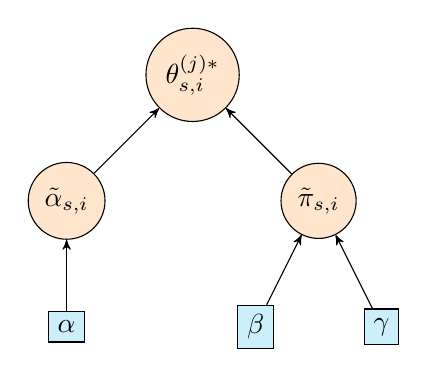
\begin{tikzpicture}
% Draw Graphical Model
   \begin{scope}[ node distance=1.6cm,on grid,>=stealth',
                   block/.style={rectangle,draw,fill=cyan!20},
                   comp/.style={circle,draw,fill=orange!20} ]
     \node [comp]  (main)                    {$\theta_{s,i}^{(j)*}$};
     \node [comp]  (c1)   [below=of main,xshift=-1.6cm]   {$\tilde\alpha_{s,i}$} edge [->] (main);
     \node [comp]  (c2)   [right=of c1,xshift=1.6cm]       {$\tilde\pi_{s,i}$} edge [->] (main);
     \node [block] (p1)   [below=of c1]       {$\alpha$} edge [->] (c1);
     \node [block] (p2)   [below=of c2,xshift=-0.8cm]       {$\beta$} edge [->] (c2);
     \node [block] (p3)   [right=of p2]       {$\gamma$} edge [->] (c2);
   \end{scope}
\end{tikzpicture}
\end{document}

%%% Local Variables: 
%%% mode: latex
%%% TeX-master: t
%%% End: 
